\section{Discussie}
\subsection{DV1: Beste classificatiemethode}
Het onderzoek behaalt resultaten in lijn der verwachting op basis van gerelateerd werk en daarnaast ruim boven de baseline scores. De lage scores voor de coalitiepartijen steunen de hypothese van een afhankelijkheid van partij-status, zoals besproken wordt in deelvraag 3. Het bijna alleen voorkomen van namen van partijen en Kamerleden in de meest karakteristieke n-grams per partij in tabel \ref{tab:MostImportantWords} steunt daarnaast het vermoeden dat deze classificatie sterk afhankelijk is van die namen, zoals besproken wordt in deelvraag 2.\par
Dit onderzoek heeft zich beperkt tot methoden genoemd in vergelijkbare onderzoeken en waarvan de implementatie beschikbaar is in scikit-learn. Een aantal methoden die in gerelateerde literatuur leidden tot goede classificaties zijn daarom niet getest. Ook nieuwe methoden die nog niet gebruikt zijn in een vergelijkbaar onderzoek voor politieke tekst classificatie zijn daarom niet getest. Daarnaast richtte zich dit ook maar op een beperkt aantal parameterwaarden. Voor vervolgonderzoek kan daarom dit onderdeel uitgebreid worden. Het effect van het beperkte aantal maximum iteraties leek bij de beste classificatiemethode beperkt.\par
Het onderzoek van Hirst et al. vond dat resultaten afhankelijk kunnen zijn van documentgrootte. Alle documenten in dit onderzoek zijn kleiner dan de grootste documentgrootte uit het onderzoek van Hirst et al. en ook de minimale documentgrootte ligt lager dan de kleinste documentgrootte uit dat onderzoek.
Het effect wat zij vinden tussen documentgrootte van 267 en 6666 is een verschil in \textit{accuracy} van 19,8\%. Dit onderzoek vindt inderdaad dat kleinere documenten vaker foutief geclassificeerd worden.
\begin{figure}[H]
  \centering
    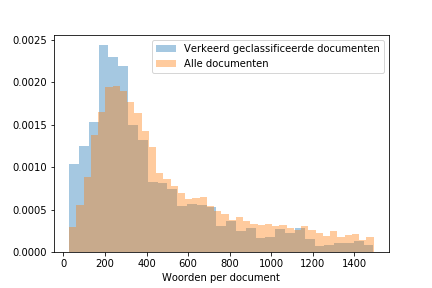
\includegraphics[width=0.40\paperwidth]{Verslag/Tables/misclassifiedlengths.png}
\caption{Genormaliseerde distributie van documentlengtes van foutief geclassificeerde documenten en alle documenten. Totaal van 5-fold cross-validation, waardoor documenten vaker voor kunnen komen. Mediaan documentlengte van foutief geclassificeerde documenten is 321 en voor alle documenten 386.}
\label{fig:misclassified}
\end{figure}
Voor een vervolgonderzoek kan uitgebreider gekeken worden naar dit effect en wat dit betekent voor de resultaten. Het percentage documenten van een vragenuur is tweemaal zo hoog bij foutief geclassificeerde documenten, maar dit lijk te komen doordat deze documenten vaak kleiner zijn (mediaan is 286).\par
Er is verder nog gekeken naar andere verbanden tussen documenten die verkeerd zijn geclassificeerd. Daarbij is nog te zien dat sprekers met weinig documenten relatief iets meer voorkomen in verkeerd geclassificeerde documenten.
Dit zou het vermoeden versterken dat de classificatie mede plaatsvindt op basis van woordgebruik van individuele sprekers, zoals besproken wordt in deelvraag 5.\par


\subsection{DV2: Invloed van namen}
De resultaten laten zien dat de classificatie sterk afhankelijk is van partijnamen en achternamen van Kamerleden. Deze daling was te verwachten op basis van gerelateerd werk.\par
De n-grams in tabel \ref{tab:MostImportantWordsWithoutNames} komen bij veel partijen overeen met hun ideologie, vooral bij one-issue partijen PVV, PvdD en 50PLUS. Daarnaast zijn er ook n-grams die niet veel over ideologie lijken te zeggen, zoals; \textit{volgens mij}, \textit{ik constateer} en \textit{in elk geval}. Vooral de SGP heeft n-grams die niet veel lijken te zeggen over de ideologie, hoewel deze partij desalniettemin de hoogste $f_1$ score heeft. Met name opvallend hierbij is \textit{mevrouw de voorzitter}, aangezien deze woorden door alle partijen gebruikt worden om via de voorzitter te praten. Voor een vervolgonderzoek kan gekeken naar waarom deze n-grams zo karakteristiek zijn voor partijen. Een hypothese is dat deze n-grams eigen zijn aan een individueel Kamerlid.\par
De classificatiemethode die gebruikt is in deze deelvraag, is gebaseerd op de beste methode voor de dataset uit deelvraag 1. Hierin was gevonden dat een combinatie van uni-, bi- en trigrams het beste resultaat opleverde. In tabel \ref{tab:MostImportantWords} is te zien dat trigrams behoren tot de meest karakteristieke n-grams, hoewel de woorden in trigrams vaak overlappen met uni- en bigrams. In tabel \ref{tab:MostImportantWordsWithoutNames} daarentegen zijn er nog maar een paar trigrams, welke grotendeels procedurele zinnen zijn of toevoeging van een lidwoord op een uni- of bigram. Dit verschil suggereert dat trigrams minder belangrijk zijn in de classificatie zonder de namen, dus de classificatiemethode uit deelvraag 1 niet het beste is voor deze classificatie. In vervolgonderzoek kan de opzet van deelvraag 1 toegepast worden op de classificatie zonder de namen, om zo te komen tot een classificatiemethode die het beste resultaat oplevert op de classificatie zonder namen.\par 

\subsection{DV3: Oppositie of regering}
In tabel \ref{tab:classrapport} is het opvallend dat de coalitiepartijen lage scores krijgen. Daarnaast laat figuur \ref{fig:confusionmatrix} zien dat er een hoge overlap zit tussen deze twee partijen.\par
De resultaten van het eerste experiment suggereren een verschil in error binnen oppositie, binnen regering en tussen deze partijen.\par
De verwachting was dat de error normaal verdeeld zou zijn.\par
De overlap van 100 meest karakteristieke n-grams tussen regeringspartijen die niet voorkomen bij oppositiepartijen gedurende kabinet-Rutte II beperkt zich tot de woorden \textit{en} en \textit{blij}, als ook \textit{toezegging} voor VVD en \textit{toezeggingen} voor PvdA.\par
\begin{table}[H]
\label{tab:overlapkabinetten}
\caption{N-grams die bij minimaal één regeringspartij in beide kabinetten voorkomen in de 100 meest karakteristieke n-grams, maar niet toen deze partijen in oppositie zaten.}
\centering
\begin{tabular}{|l|l|l|l|}
\toprule
&&\multicolumn{2}{c|}{Kabinet-Rutte II} \\ \hline
      &&   PvdA &    VVD\\ \hline

\parbox[t]{2mm}{\multirow{4}{*}{\rotatebox[origin=c]{90}{Kabinet-Balkenende IV}}}&         CDA &    \makecell[l]{\textit{toezeggingen}\\\textit{hun}\\\textit{collega KAMERLID}\\\textit{in}\\\textit{aanpak}\\\textit{collega}} &            \makecell[l]{\textit{algemeen}\\\textit{algemeen overleg}\\\textit{toezegging}\\\textit{helder}\\\textit{overleg}\\\textit{aangegeven}\\\textit{voor}\\\textit{voor PARTIJ}} \\ \cline{2-4} 
 &ChristenUnie &  \makecell[l]{\textit{mijn}\\\textit{waarop}\\\textit{blij}\\\textit{collega KAMERLID}\\\textit{erg}} &        \makecell[l]{\textit{gaan}\\\textit{termijn}\\\textit{blij met de}\\\textit{volgens}\\\textit{volgens mij}\\\textit{blij}\\\textit{beantwoording}}  \\ \cline{2-4} 
  &PvdA &   & \makecell[l]{\textit{volgens}\\\textit{volgens mij}}           \\
\bottomrule
\end{tabular} 
\end{table}
Hoewel er een aantal overeenkomsten zijn qua meest karakteristieke n-grams tussen regeringspartijen van de twee kabinetten, lijkt dit beperkt. De meeste overeenkomsten lijken daarnaast niet heel inhoudelijk gerelateerd aan partij-status. Deze resultaten suggereren daarom ook maar een beperkte invloed van partij-status op de classificatie. Voor een vervolgonderzoek kan uitgebreider gekeken worden naar de overlappende meest karakteristieke n-grams en wat deze zeggen over een regeringspartij.\par
De scores in tabel \ref{RegeringOppositie} laten een duidelijke daling zien ten opzichte van een classificatie van alleen kabinet-Rutte II. Deze algemene daling kan verklaard worden door verschuiving in ideologie, verschil in woordgebruik en/of verandering van onderwerpen. De daling is het grootst bij VVD, maar valt mee bij de twee andere partijen die gewisseld zijn van partij-status, ChristenUnie en CDA. Daarnaast is de daling ook heel sterk bij oppositiepartijen GroenLinks en D66, alsook de regeringspartij in beide kabinetten, PvdA. Dat de daling niet consequent groter is bij partijen die gewisseld zijn van partij-status, suggereert dat de invloed van partij-status beperkt is op de classificatie.\par
Dat de experimenten uit Hirst et al. in hun onderzoek wel invloed vinden, maar in dit onderzoek niet kan komen doordat hun onderzoek zich richt op binaire classificatie, terwijl dit onderzoek meerdere partijen heeft. Zo kan het ontbreken van gemeenschappelijke n-grams komen doordat regeringspartijen zich ook van elkaar moeten onderscheiden in dit onderzoek, waarvoor n-grams die relevant zijn voor partij-status weinig effect hebben, terwijl in het onderzoek van Hirst et al. de regeringspartij alleen onderscheiden hoeft te worden van de oppositiepartij. Daarnaast verklaren zij dat een daling tussen twee zittingsperioden met een wisseling van partij-status het gevolg is van deze wisseling, terwijl in dit onderzoek gekeken kan worden naar dit effect voor partijen die wel en niet gewisseld zijn.\par

\subsection{DV4: Links of rechts}
Er zijn verschillende visies op links en rechts, en de indeling van de partijen, ook buiten de twee methoden gekozen in dit onderzoek.\par

\subsection{DV5: Woordgebruik van sprekers}
De resultaten uit tabel \ref{tab:rapporttaalgebruik} zijn laag, amper hoger dan de baseline. Dit suggereert inderdaad dat eerdere classificaties in grote mate toch afhankelijk waren van het woordgebruik van sprekers. Dit is opmerkelijk aangezien vergelijkbare werken dit effect niet vinden. De meest karakteristieke n-grams van deze classificatie wijken daarnaast grotendeels niet af van die uit tabel \ref{tab:MostImportantWordsWithoutNames}.\par
Een alternatieve verklaring is dat de classificatie nu mede op basis van woordvoerderschap is. Per onderwerp heeft een partij vaak maar één woordvoerder, met uitzonderingen van wijzigingen in de fractie. Het is aannemelijk dat het taalgebruik afhankelijk is van woordvoerderschap, aangezien er andere termen gebruikt worden bij bijvoorbeeld een debat over zorg dan bij een debat over onderwijs. Stel dat documenten van een spreker in de test set geclassificeerd moeten worden, dan kan het zijn dat deze meer karakteristieke vertoont met een andere partij, aangezien er geen woordvoerder van die partij en dat onderwerp in de training set zit, maar mogelijk wel van een andere partij. Een vervolgonderzoek kan kijken of dit een verklaring is.\par

\subsection{Algemeen}
Het vergelijken van deze resultaten met vergelijkbaar werk is problematisch, aangezien de keuzes en eigenschappen van hun onderzoek het niet een één-op-één vergelijking maken. Voorbeelden hiervan zijn de documentgrootte, baselines, behouden of weglaten van namen, een spreker als document zien en het trainen en testen op dezelfde spreker. Hoewel de resultaten dus lager zijn dan die uit vergelijkbaar werk, moet hiermee rekening gehouden worden. Een vervolgonderzoek zou daarom dit onderzoek kunnen reproduceren op een ander parlement om daarmee te kunnen vergelijken.\par
Dit onderzoek richtte zich hoofdzakelijk op de Handelingen gedurende kabinet-Rutte II. Om te kijken in hoeverre het mogelijk is om deze conclusie door te trekken naar de algemene Handelingen van de Tweede Kamer, kan er in vervolgonderzoek gekeken worden naar meerdere zittingsperioden. Ook kan gekeken worden naar veranderingen als een kabinet demissionair is.\par